\documentclass[a4paper, 12pt]{article}

%\usepackage[portuges]{babel}
\usepackage[utf8]{inputenc}
\usepackage{amsmath}
\usepackage{indentfirst}
\usepackage{graphicx}
\usepackage{epstopdf}
% Para poder incluir imagens a parti de arquivos .pdf
\usepackage{pdfpages}
% Para poder ter tabelas com colunas de largura auto-ajustável
\usepackage{tabularx}
% Para ter células em tabelas que ocupam mais de uma linha
\usepackage{multirow}



\usepackage{ae}
% Para adicionar marcadores no arquivo.
\usepackage[colorlinks=true,linkbordercolor={1 1 1},urlbordercolor={1 1 1},urlcolor=blue,linkcolor=black]{hyperref}
\setcounter{tocdepth}{5}
\usepackage{bookmark}
%\bookmarksetup{open,numbered}
% Para usar fontes standard ao invés das do LaTeX (gera melhores PDFs)
\usepackage{pslatex}
% Para a hifenização em português
\usepackage[portuges, brazil]{babel}
% Para que os primeiros parágrafos das seções também sejam indentados
\usepackage{indentfirst}
% Para poder desenha diagrams de blocos de controle
%\usepackage[portuguese,noprefix,refeq,refpage]{nomencl}
% Para permitir espaçamento simples, 1 1/2 e duplo
\usepackage{setspace}
% Para quebrar equações longas
\usepackage{breqn}
% Para poder usar o ambiente "comment"
% Para poder ter tabelas com colunas de largura auto-ajustável
\usepackage{afterpage}
% Para formatar URLs (endereços da Web)
\usepackage{url}

\usepackage{booktabs}

\usepackage{float}
\usepackage{epstopdf}

% Para ajustar a aparencia dos contadores de uma enumeracao
\usepackage{enumerate}

% Para reduzir os espaços entre os ítens (itemize, enumerate, etc.)
% Este pacote não faz parte da distribuição padrão do LaTeX.
\usepackage{lib/noitemsep}
% Para as citações bibliográficas
\usepackage[alf,abnt-etal-cite=2,abnt-etal-list=0,abnt-etal-text=it,versalete,bibjustif]{abntex2cite}

\usepackage{listings}
\usepackage{color}
\definecolor{verdef}{RGB}{35,142,35}
\definecolor{roxdef}{RGB}{137,23,95}

%% newcommand define novos comandos, que podem passar a ser usados da
% mesma forma que os comandos LaTeX de base.

% Implicação em fórmulas
\newcommand{\implica}{\quad\Rightarrow\quad} %Meio de linha
\newcommand{\implicafim}{\quad\Rightarrow}   %Fim de linha
\newcommand{\tende}{\rightarrow}
\newcommand{\BibTeX}{\textsc{B\hspace{-0.1em}i\hspace{-0.1em}b\hspace{-0.3em}}\TeX}

% Fração com parentesis
\newcommand{\pfrac}[2]{\left(\frac{#1}{#2}\right)}

% Transformada de Laplace e transformada Z
%\newcommand{\lapl}{\makebox[0cm][l]{\hspace{0.1em}\raisebox{0.25ex}{-}}\mathcal{L}}
\newcommand{\lapl}{\pounds}
\newcommand{\transfz}{\mathcal{Z}}

% Não aparecer o número na primeira página dos capítulos
\newcommand{\mychapter}[1]{\chapter{#1}\thispagestyle{empty}}

% Os capítulos sem número
\newcommand{\mychapterast}[1]{\chapter*{#1}\thispagestyle{empty}
\chaptermark{#1}
\afterpage{\markboth{\uppercase{#1}}{\rightmark}}
\markboth{\uppercase{#1}}{}
}

% Seções sem número
\newcommand{\mysectionast}[1]{\section*{#1}
\addcontentsline{toc}{section}{#1}
\markright{\uppercase{#1}}
}

% No tabularx, as celulas devem ser centradas verticalmente
\renewcommand{\tabularxcolumn}[1]{m{#1}}

% Células centralizadas horizontalmente no tabularx
\newcolumntype{C}{>{\centering\arraybackslash}X}

%% Abrevia figuras e tabelas
%\def\figurename{Fig.}
%\def\tablename{Tab.}

%% No tabularx, as celulas devem ser centradas verticalmente
% No tabularx, as celulas devem ser centradas verticalmente
\renewcommand{\tabularxcolumn}[1]{m{#1}}

% Células centralizadas horizontalmente no tabularx
\newcolumntype{C}{>{\centering\arraybackslash}X}


\begin{document}
%\maketitle

\begin{titlepage}
	
	\small
	\begin{tabularx}{\linewidth}{@{}l@{}C@{}r@{}}
		% A figura foi colocada dentro de um parbox para que fique verticalmente
		% centralizada em relação ao resto da linha
		\parbox[c]{2cm}{
\includegraphics[width=\linewidth]{UFRN}} &
		\begin{center}
			\textsf{\textsc{Universidade Federal do Rio Grande do Norte\\
					Centro de Tecnologia\\
					Departamento de Engenharia de Computação e Automação}}
		\end{center} &
		\parbox[c]{2cm}{
\includegraphics[width=\linewidth]{DCA}}
	\end{tabularx}
    
    \vspace{3,5cm}
	\vfill
	\begin{center}
		  \textbf{\LARGE{MANUAL DE UTILIZAÇÃO DO \textit{TMS320C6713 DSP Starter Kit} (DSK)}}\\
		  %\title{{\large{Título}}}
		  
	\end{center}
	
	\vfill
	
	\begin{flushleft}
		\begin{tabbing}
			Desenvolvedor: \\
			Eng\textordmasculine{ } M.Sc. Jean Mário Moreira de Lima\\
	\end{tabbing}
 \end{flushleft}
	\vspace{1cm}
	
	\begin{center}
		\vspace{\fill}
			 Setembro\\
		 2018
			\end{center}
\end{titlepage}
%%%%%%%%%%%%%%%%%%%%%%%%%%%%%%%%%%%%%%%%%%%%%%%%%%%%%%%%%%%

% % % % % % % % %FOLHA DE ROSTO % % % % % % % % % %

% % % % % % % % % % % % % % % % % % % % % % % % % %
\newpage
\tableofcontents
\thispagestyle{empty}

\newpage
\pagenumbering{arabic}
% % % % % % % % % % % % % % % % % % % % % % % % % % %
\section{Introdução}

O \textit{TMS320C6713 DSP Starter Kit} (DSK) desenvolvido em conjunto com a \textit{Spectrum Digital} é uma plataforma de desenvolvimento de baixo custo projetada para acelerar o desenvolvimento de aplicações de alta precisão baseadas na geração DSP de ponto flutuante da TI (\textit{Texas Instruments}). O kit usa comunicações USB para funcionalidade \textit{plug-and-play} e um software completo para desenvolvimento, o \textit{Code Composer Studio}\texttrademark(CCS) \textit{Integrated Development Environment} (IDE).

\begin{figure}[htbp!] 
	\begin{center}
		% fbox faz uma borda ao redor do seu argumento
		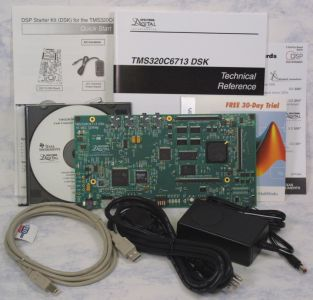
\includegraphics[scale=2]{dsp_starter_kit.jpg}
		\caption{\textit{TMS320C6713 DSP Starter Kit} (DSK)}
		\label{Fig:dskdsp}
	\end{center} 
\end{figure}

O DSP TMS320C6713 é um dispositivo de 225 MHz que fornece até 1800 milhões de instruções por segundo (MIPs) e 1350 MFLOPS. Essa geração de DSP foi projetada para aplicativos que exigem alta precisão. O C6713 é baseado na plataforma DSP TMS320C6000 projetada para as necessidades de aplicações de alta precisão e desempenho, como pró-áudio, médica e diagnóstico. Outros recursos de hardware da placa incluem:

\begin{itemize}
	\item Suporte JTAG embarcado via USB
	\item Codec estéreo de 24 bits de alta qualidade
	\item Quatro conectores de áudio de 3,5 mm para microfone, entrada de linha, alto-falante e saída de linha
	\item Flash de 512K e 16 MB de SDRAM
	\item Conector da porta de expansão para módulos plug-in
	\item Interface padrão IEEE JTAG integrada 
	\item Fonte de alimentação universal de + 5V
\end{itemize}


\newpage
\section{Primeiros Passos}

Nesta seção, explica-se brevemente os passos iniciais para utilização da placa DSP.


\subsection{Ligando a placa}

Para ligar a placa corretamente, conecte a fonte presente no \textit{Starter Kit} a placa. Uma vez que a fonte é conectada, o POST (\textit{Power On Self Test}) é executado. Os LEDs 0-3 piscarão. Quando o POST é terminado com sucesso, todos os LEDs piscam ON e OFF e permanecem ON.

\begin{figure}[htbp!] 
	\begin{center}
		% fbox faz uma borda ao redor do seu argumento
		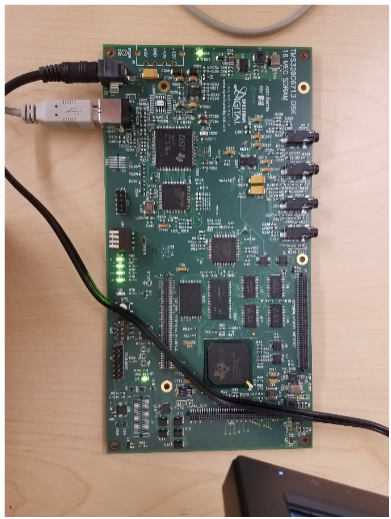
\includegraphics[scale=0.45]{dsp_on.png}
		\caption{\textit{TMS320C6713 DSP board}}
		\label{Fig:dspon}
	\end{center} 
\end{figure}

A partir desse ponto, a placa DSP está funcional e você pode conectá-la ao computador com o cabo USB também presente no kit. Agora, os próximos passos são criar, compilar e executar um projeto na placa utilizando o software de desenvolvimento \textit{Code Composer\texttrademark}.


\subsection{Desenvolvimento no \textit{Code Composer\texttrademark}}

\subsubsection{Criando um Projeto no CCS}

\begin{enumerate}
\item Para criar um novo projeto no CSS: \textbf{File->New->CCS Project}.
\item A caixa de diálogo de um novo projeto vai abrir. Preencha as seguintes configurações:

 \begin{enumerate}
 	\item \textbf{Target}: C671x Floating-point DSP / TMS320C6713
 	\item \textbf{Connection}: Spectrum Digital DSK-EVM-eZdsp onboard USB Emulator
 	\item \textbf{Project Name}: Escolha o nome do seu projeto
 	\item \textbf{Compiler Version}: TI V7.4.24 (versão instalada no CCS)
 \end{enumerate}
 
 \begin{figure}[htbp!] 
 	\begin{center}
 		% fbox faz uma borda ao redor do seu argumento
 		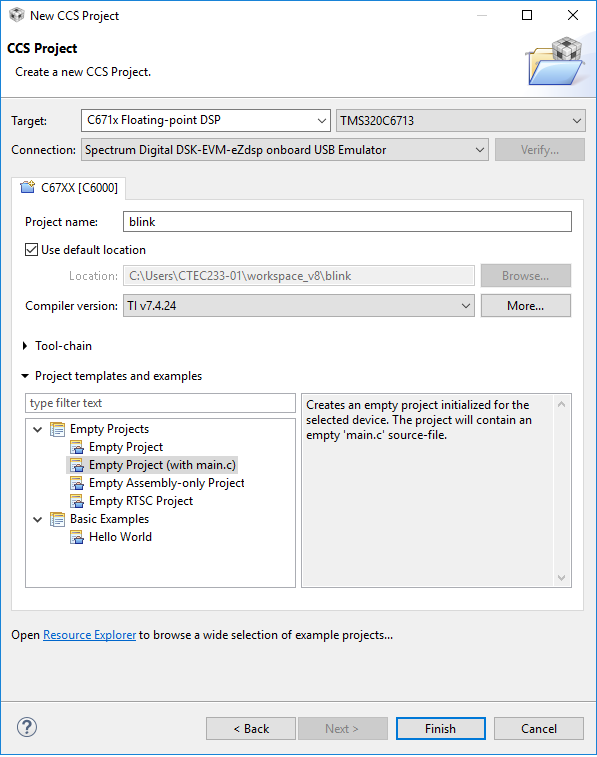
\includegraphics[scale=0.7]{css_new_project.png}
 		\caption{\textit{New Project Dialog Box}}
 		\label{Fig:dsproject}
 	\end{center} 
 \end{figure}
 
 \item Clique em \textbf{Finish} para criar o projeto.
 
 \item Agora é preciso "linkar" as bibliotecas com os códigos necessários para aplicações na DSP. Na janela \textit{Project Explorer}, clique o botão direito no seu projeto e depois em \textbf{Show Build Settings}.
 
 \item Uma noca caixa de diálogo vai aprecer. Clique \textbf{Build->C6000 Linker->File Search Path} ao lado esquerdo da janela. Acima da primeira caixa de texto, clique no ícone que é semelhante a uma folha com um sinal de mais (+) verde para adicionar a biblioteca. Digite \textbf{dsk6731bsl.lib} e clique Ok.
 
  \begin{figure}[htbp!] 
  	\begin{center}
  		% fbox faz uma borda ao redor do seu argumento
  		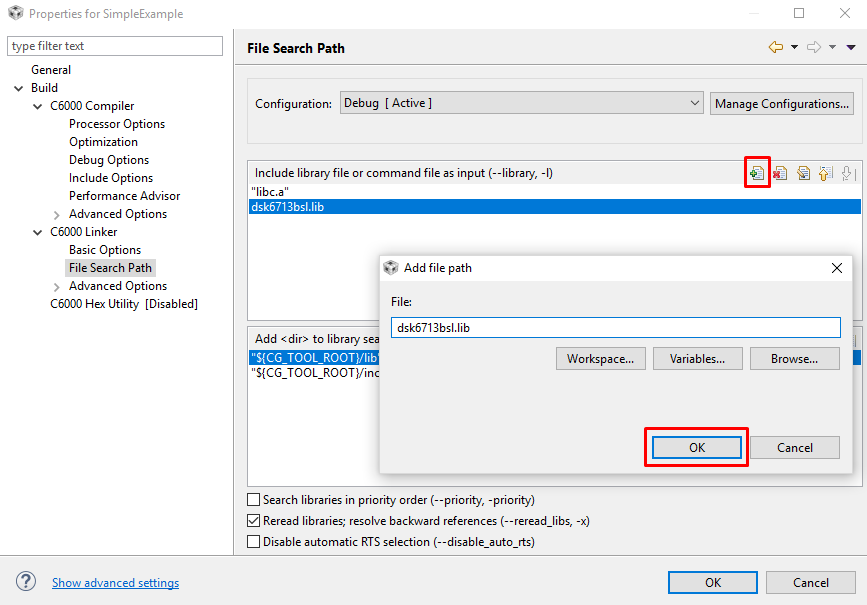
\includegraphics[scale=0.5]{linker_bib.png}
  		\caption{\textit{Adicionando Bibliotecas}}
  		\label{Fig:dspbibs}
  	\end{center} 
  \end{figure}
  
  \item Repita o passo 5 para adicionar outra biblioteca chamada: \textbf{csl6713.lib}.
  
  \item Na opção \textbf{Configuration} altere a opção \textit{Debug|Active} para \textit{Release}. Adicione as mesmas bibliotecas de antes repetindo os passos 5 e 6. Após isso, altere mais uma vez o campo \textbf{Configuration} de volta para \textit{Debug|Active}. Clique em \textbf{Apply and Close}.


\end{enumerate}

\subsubsection{Programação no CCS}

Para ilustrar a programação no CCS, vamos utilizar um exemplo:

\newcommand{\estiloJava}{
	\lstset{ %
		language=Java,                     % the language of the code
		basicstyle=\small\ttfamily,  
		backgroundcolor=\color{white},  % choose the background color. You must add \usepackage{color}
		showspaces=false,               % show spaces adding particular underscores
		showstringspaces=false,         % underline spaces within strings
		showtabs=false,                 % show tabs within strings adding particular underscores
		frame=single,                   % adds a frame around the code
		rulecolor=\color{black},        % if not set, the frame-color may be changed on line-breaks within not-black text (e.g. commens (green here))
		tabsize=2,                      % sets default tabsize to 2 spaces
		captionpos=b,                   % sets the caption-position to bottom
		breaklines=true,                % sets automatic line breaking
		breakatwhitespace=false,        % sets if automatic breaks should only happen at whitespace
		title=\lstname,                 % show the filename of files included with \lstinputlisting;
		% also try caption instead of title
		keywordstyle=\color{roxdef},      % keyword style
		commentstyle=\color{verdef},   % comment style
		stringstyle=\color{blue},      % string literal style
		escapeinside={\%*}{*)},         % if you want to add a comment within your code
		morekeywords={*,...},
		inputencoding=utf8,
		extendedchars=true        % if you want to add more keywords to the set
	}}
	
\estiloJava
\begin{lstlisting}
/*
* main.c
*/
#define CHIP_6713

#include "dsk6713.h"
#include "dsk6713_led.h"
#include "dsk6713_flash.h"

void main(void)
{
	DSK6713_init();
	DSK6713_LED_init();

	while (1)
	{
		DSK6713_LED_toggle(2);
		DSK6713_waitusec(1000000);
	}
}
\end{lstlisting}


Ao se criar um projeto no CSS, por padrão, um arquivo \textit{main.c} é criado. Na paleta \textit{Project Explorer} é possível encontrá-lo. Abra o arquivo \textit{main.c} do seu projeto e cole o código-exemplo desse material.

\begin{enumerate}
	\item A instrução \textit{\#define CHIP\_6713} é necessária para TODO e QUALQUER projeto para que as bibliotecas reconheçam que placa será usada.
	\item Para importar as funções utilizadas nesse exemplo, é preciso incluir três arquivos \textbf{dsk6713.h, dsk6713\_led.h, dsk6713\_flash.h}. De acordo com as funções necessárias ao seu projeto, é preciso importar os arquivos .h (\textit{headers}) as classes onde as funções estão implementadas.
	\item Nos seus projetos futuros, lembre-se de chamar a função: \textit{DSK6713\_init()} e outras funções \textit{init's} necessárias.
	\item Nesse exemplo, o LED 2 vai piscar a uma taxa de 1Hz.
\end{enumerate}

Após copiar o código do exemplo no seu arquivo \textit{main.c}:

\begin{enumerate} 
	\item Click no ícone similar a um martelo para construir o binário do seu código, com extensão .out. Você vai saber se a construção foi feita com sucesso se os panéis \textbf{Console} e \textbf{Problems} não exibirem algum(s) erro(s).
	\begin{enumerate}
		\item Em caso de erro relacionado com "\textit{undefined reference...}", quer dizer que, provavelmente, você cometeu algum erro no momento de lincar as bibliotecas (.lib).
		\item Em caso de erro relacionado com "\textit{cannot find some include .h file}", quer dizer que, provavelmente, você esqueceu de copiar os arquivos de \textit{include} nos diretórios corretos.
		
		  \begin{figure}[!htbp] 
		  	\hspace{-15pt}
		  	% fbox faz uma borda ao redor do seu argumento
		  	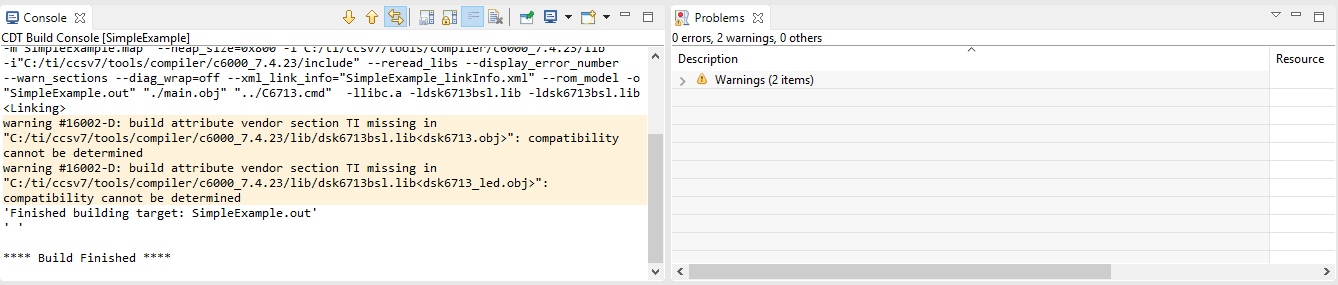
\includegraphics[scale=0.32]{console_problems.png}
		  	\caption{Tela de \textit{Console e Problems}}
		  	\label{Fig:dspconsole}
		  	
		  \end{figure}
	\end{enumerate}
	\item Finalmente, agora vamos fazer carregar o código binário na placa e rodá-lo. Clique em \textbf{Run->Debug} ou pressione \textbf{F11}.
	
	\begin{enumerate}
		\item CSS vai mudar do modo \textit{edit} para o \textit{run}.
		\item O painel \textbf{Debug}, você deve ver o nome do emulador e entre parênteses: (\textbf{Suspended - SW Breakpoint}). Isso significa que o binário foi carregado com sucesso e está esperando para ser executado.
		
		\begin{figure}[!htbp] 
			%\hspace{-15pt}
			% fbox faz uma borda ao redor do seu argumento
			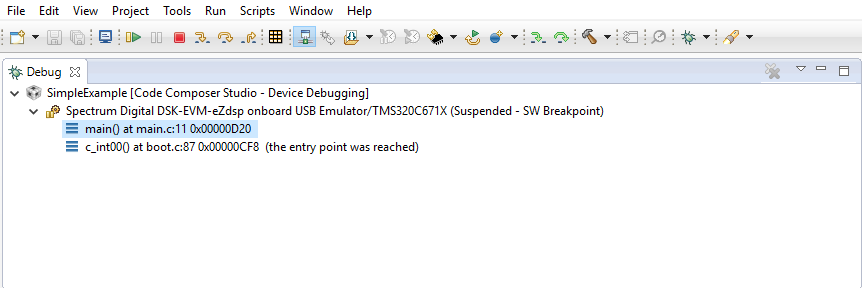
\includegraphics[scale=0.42]{waittorun.png}
			\caption{Tela de \textit{Debug}}
			\label{Fig:dspwaittorun}
			
		\end{figure}
		
		\item Clique no botão \textbf{Resume} ou pressione \textbf{F8}. Agora, seu código deve estar rodando e o painel \textbf{Debug} deve mostrar (\textit{Running}).
	\end{enumerate}
	
	\item Quando for necessário fazer mudanças no seu código e testá-lo novamente, não há a necessidade de executar todos esses passos novamente. Você pode seguir as instruções seguintes:
	
	\begin{enumerate}
      	\item Clique no botão \textbf{Suspend} ou pressione \textbf{Alt+F8}.
		\item Agora, você pode alterar seu código. Por fim, pressione o botão \textbf{Build}. Clique em \textbf{Yes} para recarregar o programa automaticamente. Assim, estará na mesma situação do item 2. Se clicar em \textbf{Resume} estará rodando seu código novamente.
	\end{enumerate}
	
\end{enumerate}

\section{Perguntas Frequentes}

\begin{enumerate}
	\item Onde posso encontrar esquemáticos, manuais técnicos e documentação do DSP?
	
	\begin{itemize}
		\item Toda a documentação necessária pode ser encontrada nesse link:\\ \url{http://c6000.spectrumdigital.com/dsk6713/revc/}
	\end{itemize}
	
	\item Como saber que funções estão disponíveis para uso?
	
	\begin{itemize}
		\item A BSL (\textit{Board Support Library}) API pode ser vista no arquivo de ajuda \textbf{C6713DSK.chm} localizado dentro do diretório \textbf{docs}. Clique duas vezes no arquivo \textbf{.chm} e o menu vai abrir:
		
		\begin{figure}[!htbp] 
			%\hspace{-15pt}
			% fbox faz uma borda ao redor do seu argumento
			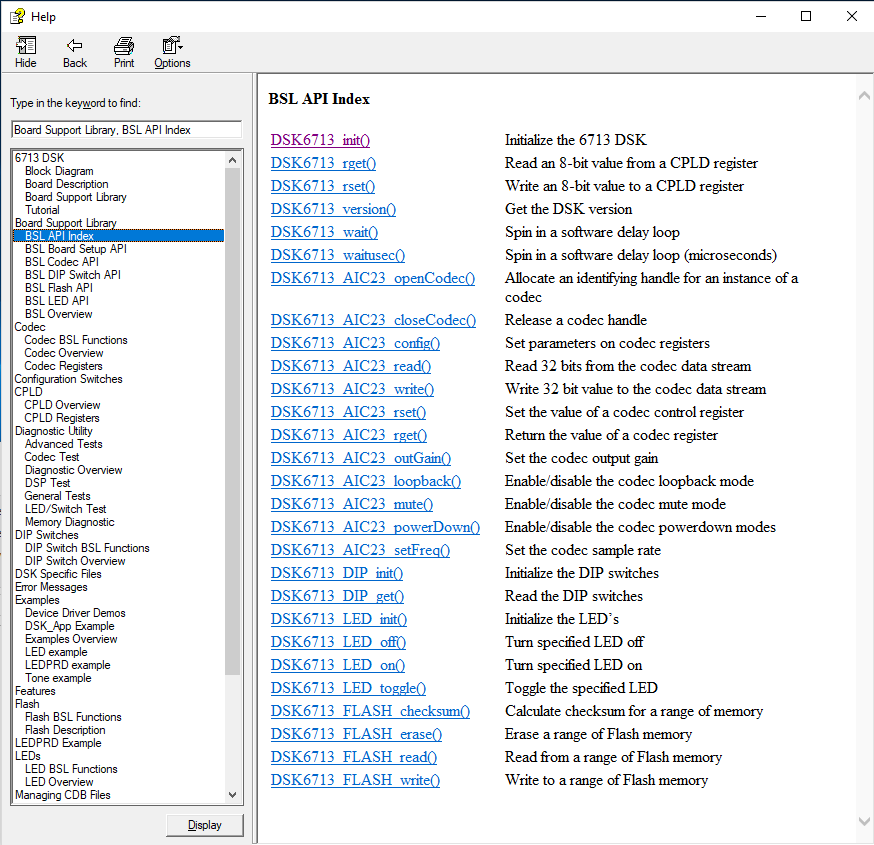
\includegraphics[scale=0.45]{bsl.png}
			\caption{Tela de \textit{Console e Problems}}
			\label{Fig:dspbsl}
			
		\end{figure}
		
		\item Além disso, todas as funções tradicionais da linguagem C estão disponíveis: \textit{free}, \textit{printf}, \\dfrac{num}{den}textit{malloc}, etc.
		
	\end{itemize}
	
\end{enumerate}


\end{document}